\chapter{Data Acquisition and Processing}
\label{ch:Data Acquisition and Processing}

While CUORE benefits from a relatively simplistic detection method compared with similar experiments in the field in that the experiment consists of effectively ~988 thermometers attached to a heat sink, converting these temperature readings to energy depositions is not a trivial process.
In particular, given that the NTDs have a strong dependence on the temperature, there are multiple sources of noise such as the pulse tubes, and data is being collected on nearly 1000 crystals simultaneously, collecting, processing, and optimizing this data requires automated and parallelizable software procedures.

\section{CUORE Data Acquisition}
Because of the need in CUORE to calibrate $\sim$monthly, there are multiple layers for how data is organized for CUORE.
At the largest scales, there are datasets that begin and end during these monthly calibrations where the closing calibration for one dataset can be used as the opening calibration for the following dataset.
Composing each dataset are runs of $\sim24$ hour length.
These runs are further broken down into 3 types: `background' for physics runs, `calibration' for calibration runs, and `test' runs.
The test runs can be much more varied in duration than the ``standard" 24-hour background and calibration runs, and can include runs for various reasons, such as setting the working points of the NTDs or for scanning pulse tube phases.

At the smallest scales, the events on each detector are similar to that shown in \autoref{fig:Sample_pulse}.
These pulses occur with rise and fall times $\approx100$ ms and $\approx400$, respectively \cite{Alduino:2017ehq}.
A 10-second window (3 seconds before and 7 seconds after) is taken around these events to understand a stable bolometer temperature before and after the event, and the amplitude of the event is used to define the energy of the pulse.
The event rate per detector is $\approx 50$ mHz and $\approx6$ mHz in calibration\footnote{With the performance of the internal and external calibration systems, this rate can vary significantly on various towers and crystals.} and physics data, respectively.
In addition, as noted in \autoref{ssec:Particle Detection with Bolometers}, there are additional thermal pulses generated by the Si heater on the crystals occurring every few minutes.
While there is a software trigger applied on these events, which is discussed more in \autoref{sec:Online Data Taking}, there is no hardware trigger on these events.
This is due to the simplicity of the detection method in CUORE, in that the only signals are purely thermal and no precise $\mathcal{O}(\mu~\textrm{s}$) timing is needed.
As a result, the data can be sampled continuously for each bolometer\footnote{Of the 988 CUORE bolometers, 4 observed an issue with the connections from the thermistor to the electronics after installation, and are unreadable.
The other bolometers have a connected signal to the NTD thermistor, while 29 of the 988 have non-functioning heaters.} at a rate of 1 kHz.

\section{Electronics Hardware and Detector Working Points}
\label{sec:Electronics Hardware}
On top of the Y-beam directly above the cryostat are the electronics hardware that reads out and biases the thermistor and Si heater electronic circuits.
These signals are carried up from the Cu-PEN tapes through the cryostat with twisted-pair constantan wires.
The NTDs are biased through two low-noise load resistors, and the voltage is measured by means of a low-noise room temperature preamplifier, a gain amplifier, and a 6-pole Thomson-Bessel low-pass filter \cite{doi:10.1063/1.4936269, PESSINA2000132, ARNABOLDI2010327}.
Lastly, these signals are digitized into a differential ADC\footnote{\RaggedRight NI PXI-6284: \url{http://sine.ni.com/nips/cds/view/p/lang/en/nid/201759}}
For each of the 988 bolometers in CUORE, the bias, gains, and offsets need to be tuned independently.
As one of the critical parameters for CUORE is the sensitivity at the \zeronubb~Q-value, maximizing the signal-to-noise ratios on each NTD is paramount.
This is achieved by first setting the bias on each of the NTDs.
At low bias, the signal amplitude depends linearly on the bias, but, at high bias, the temperature of the NTD increases, which affects the resistance and sensitivity of the NTD to signal.
In addition, different levels of bias induce various other effects on the noise, and the signal-to-noise ratio is not necessarily maximized when the amplitude is maximized.
In these scenarios, the bias is set to be when the Signal-to-Noise Ratio (SNR) is maximized which is generally higher than the bias that maximizes the amplitude.
However, if the SNR is maximized, but a high bias makes the baseline unstable, the bias is instead lowered to the bias that maximizes the amplitude \cite{Lucia:LoadCurvesDoc}.
Following setting the bias for each channel, the gain and offset are then set for each channel such that a 2615 keV signal returns a 1-2 V amplitude and that events with energies up to 10-20 MeV can be recorded.
Given that the ADC range is -10 V to 10 V, an offset of $-4$ to $-7$ V is used which allows for the higher-energy events to be observed, while preventing a drifting baseline from saturating the ADC low.
This setting of bias, gain, and offset for each channel is called a working point, and these working points are generally held constant between datasets\footnote{In the event of a warm-up between datasets or in the case of changing the operating temperature of CUORE, these values need to be redetermined.}.
Lastly, the electronics hardware also assigns tower and channel numbering to all the detectors in CUORE, as shown in \autoref{fig:DAQ_tower_numbering}.

\begin{figure}
    \centering
    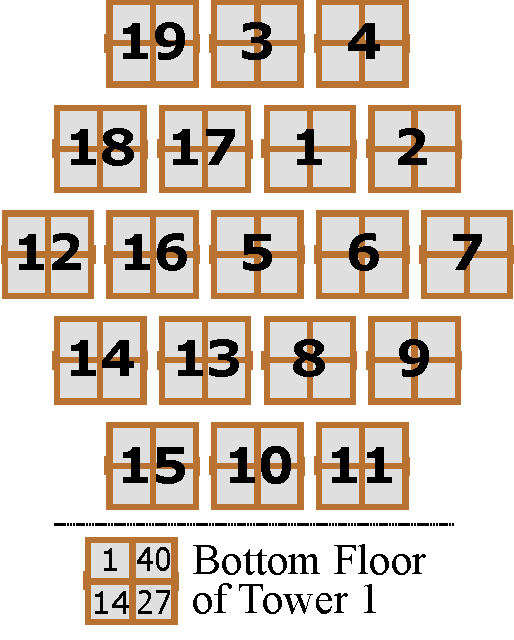
\includegraphics[width=0.5\linewidth]{Figures/Crystals_numbering_only.pdf}
    \caption[The tower and channel numbering from the Data Acquisition System.]
    {The tower and channel numbering from the Data Acquisition System.
    The arrangement of the towers is the same as shown in \autoref{fig:Calibration_source_locations}.
    In addition, the channels on each tower are numbered vertically from the bottom to the top (1-13, 14-26, etc.) along each column counter-clockwise from the top-left.}
    \label{fig:DAQ_tower_numbering}
\end{figure}

\section{Online Data Taking}
\label{sec:Online Data Taking}
The software used to collect the CUORE data is the \textsc{Apollo} software package that controls the working point setup and reading and triggering on data.
During data-taking, events can be categorized into three categories.
The first type of events are the physics events that consist of particles depositing energy in the crystals.
The second type of events are the heater pulses that occur on every channel every 380 seconds.
Lastly, the third type of events are noise events that occur without the presence of any significant energy deposition or Si heating. 
\subsection*{Signal Triggering}
There are two triggers used in CUORE to detect thermal events in the detectors.
The Derivative Trigger is the trigger used in standard analyses that triggers when the derivative of the baseline exceeds a certain threshold for long enough.
This threshold is set for each channel to be as low as possible before triggering excessively on noise events\footnote{If the threshold is set too low, this excessive event rate can crash the Data Acquisition System.
In addition, earthquakes can also cause the trigger to fire excessively and cause a crash.}, and, in addition, a 1 second dead time is placed on each channel before another signal may be triggered although a longer 10 second window is placed later on in the analysis.
These thresholds generally occur at $50-100$ keV per channel.
For triggering on lower-energy events, another trigger called Optimum Trigger is used, which utilizes a filtered waveform to reduce noise and suppress noise-induced pulse shapes that allows for $<10$ keV thresholds.
However, only the Derivative Trigger is used in this analysis as the events of interest occur at energies above 100 keV. 
These triggered events are classified then in three ways.
Firstly, the events that cause the Derivative Trigger to fire are labelled as the signal events described above.
For events that are due to the Si heaters on a channel, these are flagged by the software as \textsc{Apollo} reads that the pulsers are firing.
These events are also used as a test of the Derivative Trigger, as the efficiency of this trigger should be 1.
Lastly, the trigger also occurs on noise events.
This is done by triggering on every channel in a tower every 80-100 s.
These noise events allow for a measurement of the energy resolution at 0 keV, as no signal should be measured in these events.
In addition, these noise events allow for a measurement of the power spectrum of the noise on the detectors, and is what is minimized during a scan of the pulse tube phases.

\section{Offline Data Processing}
After the data are collected, the real work of processing can begin.
Again, all the data collected by CUORE directly comes in the form of an output voltage measured by the NTD.
The following processing steps are used to convert this data into a finalized format detailing the deposited energies of the particles that interact in the detectors, along with any associated energy depositions in other crystals, while optimizing signal resolution.
This processing is done with a special software developed for CUORE called \textsc{Diana} and is done in a set of ordered steps over all the triggered data.
First, the data is preprocessed to determine both the number of pulses in a trigger and the baseline slope in an event. 
Then the heights of the pulse peaks is determined and the baselines are stabilized.
Later, these stabilized amplitudes are mapped to a calibration spectrum and assigned an energy.
For energies near the \zeronubb Q-value, and 2615 keV peak, these energies are also salted and blinded in the \zeronubb~analysis.

\subsection*{Assigning Energies to Pulses}
The first steps of processing are to assign energies to the pulses and then applying the blinding of the \zeronubb~ROI.
While this blinding is applied in every step of the analysis chain after energies are assigned, this blinding procedure is not performed for the background model and Majoron searches, and will not be discussed in this thesis.

\subsubsection*{Bad Intervals}
Firstly, after the data is collected by \textsc{Apollo}, bad intervals are then applied to the data to subtract out times when the data are noisy or otherwise unsuitable for analysis, such as when the baselines saturate low or high, when a mechanical or electronic malfunction causes instability of the detector baseline, or during an earthquake.
Depending on the source of the issue, these bad intervals can be set channel-by-channel or detector-wide, and can be set either by an automatic tool that detects these times, or manually by an analysis shifter.

\subsubsection*{Preprocess}
Before processing each event, we first ``preprocess" to determine the detector state before the event occurs and to determine how many pulses are included in each trigger.
This is done by fitting the first 2.25 seconds of the data before a trigger and fit a line to determine the average baseline and the baseline slope.
In addition, the baseline noise is defined as the RMS of the data.
Then, the number of pulses in the event is determined by taking a smoothed derivative of the pulse and searching for locations where the derivative is over 5 times that of the RMS with only positive pulses counted.

\subsubsection*{Amplitude Evaluation}
Next, the amplitude of each event is calculated through a modeled waveform,
\begin{align}
    v_i(t) = \bar{A}_i\cdot s_i(t) + n_i(t) + b
    \label{eq:pulse function}
\end{align}
for each bolometer $i$ where $\bar{A}_i$ is the amplitude of the pulse, $s_i(t)$ is the signal response, $n_i(t)$ is the noise, and $b$ is the baseline \cite{Alduino:2016zrl}.
The amplitude $A$ can, to good approximation, be considered as
\begin{align}
    \bar{A}_i = G_i(T)\cdot A_i(E)
\end{align}
with $G_i(T)$ being the bolometric gain due to the temperature of the NTD and the setting of the working point, and $A_i(E)$ being the ``true" energy-dependent amplitude of the pulse from an energy deposition.
To determine the signal response, a ``standard" set of pulses are used to evaluate an averaged pulse.
This averaging is done with two sets of data: first, the heater pulses are used, and then, after the channels have been calibrated, pulses at the $^{208}$Tl 2615 keV peak are used.
Average pulses are determined by taking the pulses in data for each channel with $>40\times$ the baseline RMS and averaging out the pulse shapes.
This averaging removes any independent noise sources in $n_i(t)$ and allows for a measurement of $s_i(t)$.
The next step is to reduce the noise term further, as the noise here directly affects the detector resolution.
This is done via an optimum filter that converts the input voltage to frequency to maximize the SNR given the $s_i$ from averaging the pulses and an average noise power spectrum from the triggered noise events \cite{Gatti1986}.
This filter takes \autoref{eq:pulse function} into frequency space as
\begin{align}
    O_i(\omega)=\frac{S_i^\star(\omega)}{N_i(\omega)}e^{i\omega t_{\textrm{max}}}V_i(\omega)
\end{align}
where $S_i(\omega)$ and $V_i(\omega)$ are the Fourier transforms of their counterparts in \autoref{eq:pulse function}, $N_i$ is the noise power spectral density, and $t_\textrm{max}$ is the time where the pulse amplitude is highest.
With this filtered pulse, the height of the pulse is extracted by finding the first maximum in the filtered pulse and fitting a 2nd-order polynomial.
This maximum is then used as the pulse amplitude\footnote{While, in principle, the pulse area could also be used to determine the energy of each pulse, using the height yields the best energy resolution.
This can be understood as the SNR is maximized as only the noise at the maximum amplitude factors into the resolution instead of integrating the noise when evaluating the pulse area.}.

\subsubsection*{Stabilization}
\label{ssec:Stabilization}

While the temperatures of the bolometers are generally quite stable over a dataset, not every pulse happens with the crystals at precisely the same temperature.
As noted previously in \autoref{ssec:Particle Detection with Bolometers} and above, the resistances of the NTDs are a function of temperature, and this directly affects the measured height of the pulses.
To resolve this issue, the Si heaters are used to provide a temperature-independent pulse that allows for a measurement of $G_i(T)$.
As the energy dissipated in the silicon heater transfers into the bolometer similarly how a real energy deposition would look in a physics event, we then apply a fixed-energy input at regular intervals \cite{ALESSANDRELLO1998454:Si-heater}.
Using these known heater pulses, a linear fit is applied to the amplitudes of these pulses relative to their baselines.
For the 29 channels where the heater is disconnected, this procedure is unavailable, so a different method is needed.
Instead of using these heater pulses, the 2615 keV $^{208}$Tl line is used from calibration data, which is done over a dataset instead of over each run as the previous method.
This causes a larger spread in the possible baselines as the variation over a month-long dataset is larger than that over a day-long run, and a 2nd-order polynomial is used to fit these baselines and amplitudes to account for the non-linearities in the temperature-dependence.
These two stabilization methods are applied to all channels, however, and later a choice is made about which method optimizes each detector's sensitivity.

\subsubsection{Calibration}
\label{ssec:Calibration}
Once each event has a baseline-independent amplitude, it can then be assigned an energy.
Using the sources described in \autoref{chap:DCS}, these amplitudes are then matched with the known spectrum of $^{232}$Th decay.
This is done by searching for the highest peak in stabilized amplitude and determine that as the 2615 keV $^{208}$Tl peak.
Afterwards, the algorithm linearly extrapolates down to each of the lower-energy peaks and searches for the bin with the highest number of counts near the expected peak.
After each peak is found, that peak is fit with a Crystal Ball function and the mean is used to update the temporary calibration function to predict the location of the subsequent peak.
As noted in \autoref{ssec:CUORE Calibrations}, not every calibration allows for all the channels to have all 6 peaks observable.
Therefore, the algorithm searches for as many peaks as possible, and, especially in the case of channels with the worst performance, \textsc{Diana} can fail to find a minimum number of peaks.
In this case, the user can manually search for the peaks and select their approximate locations for the software to then fit.
Once this procedure has been fully performed, a final calibration function is fit for each channel by using a 2nd-order polynomial with zero intercept, and thus an energy can be assigned to each event occurring in each bolometer.

\subsection*{Data Selection and Labelling}
After energies have been assigned to each event, then the next layer of analysis can begin.
In this part of the analysis, other labels are assigned to an event, in particular, the data is selected for quality with pulse shape analysis cuts and events are assigned a multiplicity which corresponds to how many detectors observe an event simultaneously.
Lastly, a decision is made about which analysis technique to use is performed at the end in order to agnostically compare different methodologies to optimize CUORE's sensitivity.

\subsubsection*{Pulse Shape Analysis}
While the response of CUORE's detectors is too slow to allow for any type of particle or surface/bulk discrimination based on the shape of the pulses, it is sufficient to allow to rejection of noisy pulses, pileup events, or energy depositions taking place in the NTD itself.
From a filtered pulse, 6 parameters are used to describe the event and limits on each of these are used to form a pulse-shape cut optimized to remove these unwanted events from the data while leaving ``good" candidate events untouched.

\begin{description}[align=left]
\item [Rise and fall times] The first parameters are based on the time it takes for the pulse to rise and fall, defined as the time it takes for a pulse to rise from 10\% to 90\% of the amplitude and for the pulse to fall from 90\% to 30\% of its maximum, respectively.
For example, a pulse that is due to a spike in detector noise may have a fast rise and fall time, while good signal pulses have rise and fall times approximately 100 and 400 ms, respectively.
\item [Baseline slope] The next parameter is the baseline slope of the event, which, as noted above in this section, is a measurement of the baseline in the first 2.25 seconds.
A good event will have a slope that is generally flat, corresponding to the detector conditions also being stable, while, e.g., an event that occurs too soon after another pulse in the same bolometer will have a falling baseline slope and will degrade a measurement of the energy of the later pulse.
\item [Peak delay] As triggered pulses have 3 seconds of data written before the trigger and it takes a good event roughly 100 ms to rise to the maximum, another parameter is the time it takes the pulse to reach the maximum from the start of the triggered window.
\item [TVL and TVR] Parameters named ``Test Variable Left" and ``Test Variable Right", effectively $\chi^2$ values for a fit between the template averaged pulse versus each pulse, are also used.
These are used on the right- and left-hand sides of the peak and determine how well the pulse matches the template, and are named.
\end{description}
Each of the distributions in each of these parameters vary across channels and datasets, and have an additional complication as they are also energy-dependent.
The solution to avoiding these complications is to normalize each of these parameters into a channel-, dataset-, and energy-independent form.
This is achieved by binning each pulse shape parameter from a single channel in each dataset according to the energy and calculating the median and median absolute deviation (MAD).
This value is then transformed into the normalized form by
\begin{align}
    \textrm{PSA}_{\textrm{norm}} = \frac{\textrm{PSA} - \textrm{Median}(E)}{\textrm{MAD}(E)}.
\end{align}
Of course, the most important part of setting these cuts is to determine what these parameters look like in ``good" signal pulses.
For this, events from the highest-occurring peaks in the background spectrum are used, namely from events within 10 keV of the peaks due to $^{40}$K at 1461 keV and $^{60}$Co at 1173 and 1332 keV.
Using events at these energies, which, while not being a 100\% pure sample of good events, have a significantly larger fraction of good events.
With these events, a mean of each normalized pulse shape parameter is determined along with a covariance matrix between all the parameters.
These 6 parameters then form a 6-dimensional space and the Mahalanobis distance is used to calculate how many standard deviations each pulse's parameters are from the mean \cite{mahalanobis1936generalized}.
This distance, $D_M$, is defined as
\begin{align}
    D_M(\Vec{x}) = \sqrt{(\Vec{x}-\Vec{\mu})^TS^{-1}(\Vec{x}-\Vec{\mu})}
\end{align}
where $\Vec{x}$ and $\Vec{\mu}$ are vectors containing the normalized parameters from a pulse and the mean of the ``good" pulses and S is the covariance matrix of these parameters.
Setting an upper limit on this allowed distance is then used as the pulse shape cut, and thus a limit of $D_M<5$ is set by optimizing the senstitivity.

\subsubsection*{Coincidence Analysis}
One of the last data to be processed is an analysis of the coincidence rates between various bolometers.
While CUORE lacks any particular particle identification through any pulse shape analysis, there is still significant background rejection that can be had through a coincidence analysis.
For example, a $\gamma$ or muon can deposit energy in multiple crystals, whereas an expected \zeronubb~or\twonubb~decay will deposit its energy in a single crystal 88\% of the time.
Therefore, this stage of the analysis seeks to label each event as being in coincidence with either 0, 1, 2, etc. other events.
However, while the events that interact with multiple crystals are significantly faster than the readout\footnote{Compare a $\gamma$ that pass through the detector region in $\mathcal{O}(10^{-9})$ seconds or a 4 MeV $\alpha$ that can pass between crystals in also in nanoseconds to the millisecond response time of the electronics.} and can be considered as instantaneous, variations in the responses of each crystal require more careful consideration.
These variations are called ``jitter" and need to be taken into account when determining the rates of ``true" versus ``accidental" coincidences between events that are truly coincident such as Compton scattering in multiple crystals versus two single-crystal events that happen to occur simultaneously, respectively.
In order to measure this jitter, calibration data with a large fraction of 2615 keV $^{208}$Tl events are used because have significantly higher rates of ``true" versus ``accidental" coincidences.
In this data, two pulses within a $\pm100$ ms window that have total energy summing up to 2615 keV should only have a timing difference due to their responses.
Therefore, when considering pulses to be simultaneous, by correcting the timing of events with this jitter, a significantly smaller coincidence window can be used\footnote{An important question that should be asked is if this is true at multiple baselines or at varying energies, but this jitter seems to be independent of these effects, greatly simplifying this analysis.}.
In the analysis, a coincidence window of $\pm5$ ms is then used to label each event with the number of simultaneous events in the detectors, viz. M1, M2, ... where M$\star$ refers to the ``multiplicity" of the event\footnote{No geometric cut is used on CUORE data, however, as it does not strongly affect the results within a 10 ms window.}.
This labelling is highly critical not only to a \zeronubb~search, but also to any measurements of the background model, as discussed in \autoref{ch:Background Model}.
In particular, the processed data are split by their multiplicities, and any misidentification of an M1 event as M2 or M2 as M3 and their reverses due to accidentals or otherwise adversely affect the accuracy of the fit. 
Lastly, events to be considered in these windows are all subject to the same pulse triggers and cuts and are such constrained to have energies $>150$ keV, and to simplify the analysis, only a single energy estimator, $E_{OF}$ is used, which will be discussed in the following.

\subsubsection*{Energy Estimator Selection}
As there are multiple ways to estimate the energy of events in CUORE due to multiple methods of processing the data, e.g. the choice of stabilizing pulse amplitudes off of the heater pulses or off of $^{208}$Tl decays, a choice needs to be made as to which estimation is used in the final analysis.
Instead of making this decision a priori or even during the analysis, the analysis is performed after performing all the steps above.
Naturally, for some channels that lack a functioning Si heater, there is not a choice of which estimator to use in this case, but, in principle when there is a choice between two estimators to use or a choice between a new analysis technique versus an older one, the following procedure, described in the case of the stabilization choice, is followed \cite{PRL2017_InternalNote}.
First, a ratio, R, is calculated according to the formula
\begin{align}
    W=\frac{t_c^2/\sigma_c^2}{t_h^2/\sigma_h^2}
\end{align}
where $t$ refers to the livetime and $\sigma$ to the resolutions of the $2615$ keV $^{208}$Tl line, and the subscripts $c$ and $h$ refer to the calibration and heater stabilizations, respectively.
Additionally, another metric, Z, is used with
\begin{align}
    Z = \frac{1-W}{\sigma_W}
\end{align}
where $\sigma_W$ is the variance of W.
With these values, $W<1$ means that the alternative energy estimator provides better performance for a particular channel, and $Z$ measures the significance of the improvement.
Returning to the stabilization example, as the heater stabilization is generally a sightly better approach for most channels, this is the baseline approach and switching to the alternative calibration stabilization approach is only performed when both $W<1$ and $Z>1$.
Finally, once this choice of energy has been made, the data processing chain has been completed with every triggered pulse selected for quality and labelled according to its energy and multiplicity.